\documentclass[journal, a4paper]{IEEEtran}
\usepackage{pgf,tikz}
\usepackage{mathrsfs}
\usetikzlibrary{arrows}
\usepackage{amsmath} 
\usepackage{amsthm} 
\usepackage{amssymb}
\usepackage[hidelinks]{hyperref}
\usepackage{graphicx} 
\usepackage{array}
\usepackage{hyperref}
\usepackage{blindtext}

\usepackage [english]{babel}
\usepackage [autostyle, english = american]{csquotes}
\MakeOuterQuote{"}


\begin{document}

\definecolor{uuuuuu}{rgb}{0.26666666666666666,0.26666666666666666,0.26666666666666666}
\definecolor{xdxdff}{rgb}{0.49019607843137253,0.49019607843137253,1}
\definecolor{qqqqff}{rgb}{0.49019607843137253,0.49019607843137253,1}
\begin{titlepage}
    \begin{center}
        \vspace*{1cm}
        
\includegraphics[width=0.4\textwidth]{logo.png}\\
        \textbf{REPORT on Bluetooth 5}
        
        \vspace{0.5cm}
        Features, Comparison and Possibilities for IoT
        
        \vspace{8cm}
        
        \textbf{Ravinath, W. A. D. A. P.}\\
        140530L
        
        \vfill
				\vfill
        
        This is submitted as a partial fulfillment for the module\\
        EN3250: Internet of Things\\
				Department of Electronics and Telecommunication Engineering\\
				University of Moratuwa\\
				25\textsuperscript{th} of January, 2018\\         
    \end{center}
\end{titlepage}


\title{Bluetooth 5-Features, Comparison and Possibilities for IoT}
	\author{Amila Pasan,\\
	Undergraduate, Electronics and Telecommunication Department, University of Moratuwa,\\
	Katubedda, Sri Lanka\\
	amilapsn@gmail.com}

\maketitle
    

\begin{abstract}
	In this report we discuss about the new version of Bluetooth Low Energy, Bluetooth version 5. Mainly we are going to focus on its new features. Then a comparison with earlier versions is discussed. In the end how Bluetooth 5 would potentially enable new possibilities for IoT is illustrated.
\end{abstract}

\begin{IEEEkeywords}
Adaptive gain control (AGC); Gaussian frequency shift keying (GFSK); Frequency hopping Spread Spectrum (FHSS); Protocol data unit (PDU)
\end{IEEEkeywords}


\section{Introduction}

	\IEEEPARstart{B}{luetooth} 5 is the newest version that was introduced to the Bluetooth family which is standardized as IEEE 802.15.1. It was released in late 2016. Bluetooth 5 included many major changes in the Bluetooth Low Energy (BLE) series. Samsung Galaxy S8, iPhone X, iPhone 8 and 8+ were some of the notable commercial early-adopters of Bluetooth 5 \cite{WIKI}. 
	
\section{New Features}

There are 4 major features of Bluetooth 5 \cite{SCHULZ}:

\begin{itemize}
\item 2x data rate to 2Msymbols/s 
\item 4x range
\item 8x broadcast capacity
\item Higher available transmit power
\end{itemize}

\subsection{2x Data Rate}

This feature is achieved through a new modulation mode. Both Bluetooth LE and Classic has a single modulation mode with Gaussian frequency shift keying (GFSK). As the nominal frequency deviation is $\pm 250~\text{kHz}$, they achieve a gross data rate of $1$ Mbps.

The new optional PHY with a nominal frequency deviation of $\pm$500 kHz has been introduces to Bluetooth 5, resulting a gross data rate of $2$ Mbps \cite{SCHULZ}.

It is important to mention that this increase in data rate is achieved without increasing the power consumption \cite{MOUSER}.

\subsection{4x Range}

This kind of a dramatic increase in range is achieved using a special kind of a coding for long range with the addition of more overhead. 

\subsubsection{Packet Format for Coded PHYs (LE Long Range)}

\begin{figure}[!hbt]
		\begin{center}
		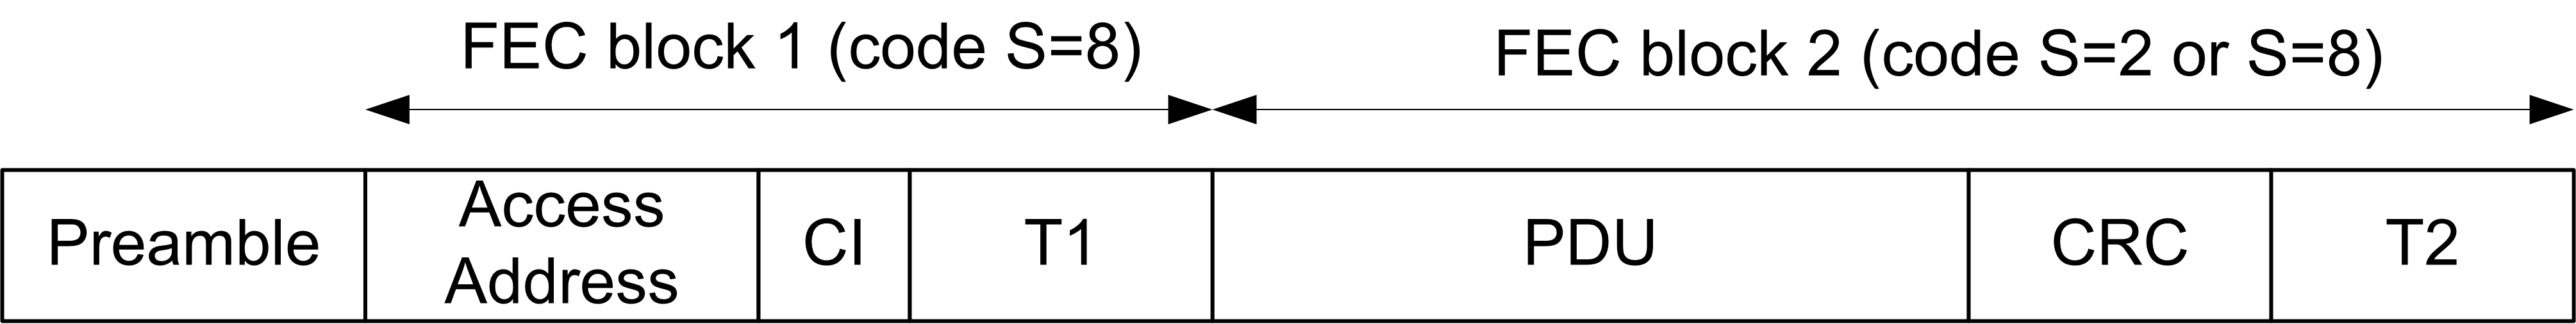
\includegraphics [width=.4\textwidth]{packet_of_coded_PHYs.png}
		\caption{Packet of coded PHYs for long range }.
		\label{fig:packet}
		\end{center}
\end{figure}

wA packet of coded PHYs for long range is shown in Fig. \ref{fig:packet}. Following items are common to long range mode and other modes.
\begin{itemize}
\item Preamble: A fixed sequence of 0s and 1s to help the receiver to synchronize, etc. and for other purposes like adaptive gain control (AGC).
\item Access address: A random value to identify access to a physical channel.
\item Protocol data unit (PDU): Actual message, for instance Tx address + Rx address + user data
\item CRC: cyclic redundancy check
\end{itemize}

Following overheads are specific to long range mode to facilitate long range communication:

\begin{itemize}
\item CI: Coding indicator is used to signal the coding block 2.
\item T1 and T2: Termination Fields are generated using a forward error correction encoder.
\end{itemize}

\subsection{8x Broadcast Capacity}

Bluetooth low energy advertising procedures are extended in order to achieve this feature.

\begin{figure}[!hbt]
		\begin{center}
		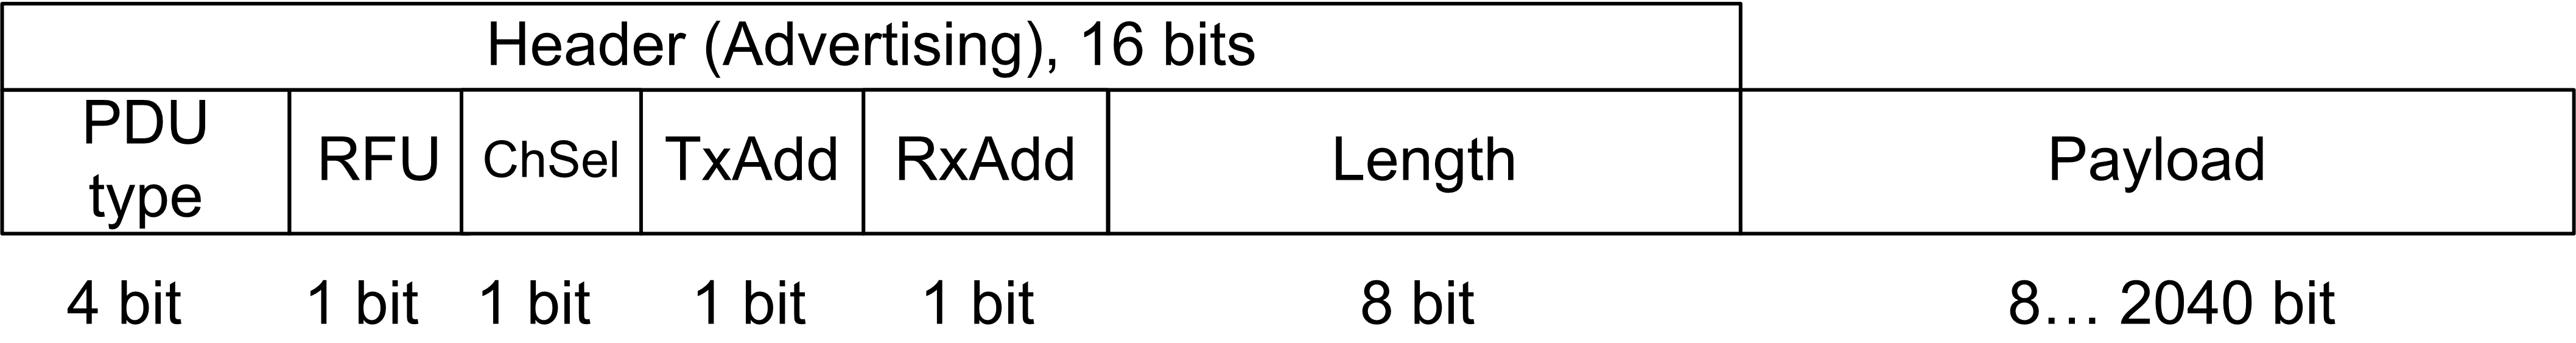
\includegraphics [width=.4\textwidth]{pdu_advertising.png}
		\caption{PDU for advertising }.
		\label{fig:advertising}
		\end{center}
\end{figure}

Advertising allows devices to broadcast information defining their intentions. It can be considered as Bluetooth communication starts with advertising \cite{ADVERTISING}.

PDUs are of 2 kinds in Bluetooth low energy in terms of transmission:
\begin{itemize}
\item data : 37 channels are dedicated 
\item advertising: 3 channels are dedicated
\end{itemize}

In Bluetooth 4.0 it was the case. But Bluetooth 5 allows the other 37 channels also for advertising, defining a secondary set of advertising channels.

Following are the new advertising PDUs defined:

\begin{itemize}
\item ADV\_EXT\_IND: Supports unconnectable (broadcast only) and scannable directed events
\item AUX\_ADV\_IND: Used for first fragment of advertising data sent on the secondary advertising channel (unconnectable and scannable directed)
\item AUX\_SYNC\_IND: Used for periodic advertising where unidirectional data is sent at fixed intervals
\item AUX\_CHAIN\_IND: Sends remaining data from incomplete auxiliary PDU advertising events
\end{itemize}

More information is available in \cite{ADVERTISING_EXTENDED}.

\subsection{Higher Available Transmit Power}

In Bluetooth 5, the avalilable transmit power can be go up to +20 dBm. To keep a low energy consumption, an independent power controller is allowed to be used in a Bluetooth 5 enabled device. Informative Tx power classesin Bluetooth Low Energy is shown in Tab. \ref{table:power-classes}.

\begin{table}[h!]
\caption{Informative Tx power classes in BLE}
\label{table:power-classes}
\centering

\begin{tabular}{||c| c||} 
 \hline
 Class & Max Output (dBm) \\ %[0.5ex] 
 \hline\hline
 1 & +20 \\ %[1ex] 
 \hline
 1.5 & +10 \\ %[1ex] 
 \hline
 2 & +4 \\ %[1ex] 
 \hline
 3 & 0 \\ %[1ex] 
 \hline
\end{tabular}


\end{table}


\section{Comparison with other Versions of Bluetooth}

\begin{table*}[]
\centering
\caption{Comparison between Bluetooth versions}
\label{table:comparison}
\begin{tabular}{||c|c|c|c||}
\hline
Feature                  & Bluetooth Classic     & Bluetooth 4.x                                                                               & Bluetooth 5                                                                                                           \\
\hline\hline
RF (MHz)                 & 2400 - 2483.5         & 2400 - 2483.5                                                                               & 2400 - 2483.5                                                                                                         \\
\hline
Range (m)                & Up to 100             & Up to 100                                                                                   & Up to 400                                                                                                             \\
\hline
Medium Access Technique  & Frequency hopping     & Frequency hopping                                                                           & Frequency hopping                                                                                                     \\
\hline
Nominal data rate (Mb/s) & 1 - 3                 & 1                                                                                           & 1 - 2                                                                                                                 \\
\hline
Latency (ms)             & $>$100                 & $>$6                                                                                         & $>$3                                                                                                                   \\
\hline
Network Topology         & Piconet, scatternet    & Star-bus, mesh                                                                              & Star-bus, mesh                                                                                                        \\
\hline
Multi-hop Solution       & Scatternet            & Yes                                                                                         & Yes                                                                                                                   \\
\hline
Nodes/Active Slaves      & 7                     & Unlimited                                                                                   & Unlimited                                                                                                             \\
\hline
Message Size (bytes)     & Up to 358             & 31                                                                                          & 255                                                                                                                   \\
\hline
RF Channels              & 79 with 1 MHz spacing & \begin{tabular}[c]{@{}l@{}}40 with 2 MHz spacing\\ * 3 advertising\\ * 37 data\end{tabular} & \begin{tabular}[c]{@{}l@{}}40 with 2 MHz spacing\\ * 3 advertising\\ * 37 data (+ secondary advertising)\end{tabular}\\
\hline
\end{tabular}
\end{table*}

Table \ref{table:comparison} compares and contrasts between Bluetooth Classic, Bluetooth 4.x and Bluetooth 5.

\section{New Possibilities for IoT}

Some use cases that emerge with new features of Bluetooth 5 are briefly discussed below:

\subsection{Technologies Related to Beacons}

Since Bluetooth 5 has such a higher broadcast capacity, the technology will be one of the most suitable candidates for beacons. Some use cases are given below:

\begin{itemize}
\item Proximity beacon: Since Bluetooth 5 has the advertising PDU ADV\_EXT\_IND which supports unconnectable (broadcast only) events these kinds of beacons can use Bluetooth 5 technology. For example suppose we are in a art exhibition. When a guest go near an art of an elephant the sound of an elephant plus information of art can be generated with these kinds of beacons

\item Maintenance beacon: ADV\_EXT\_IND also supports scannable directed events. For example, a bathroom beacon broadcasting directly to a central controller of an apartment. The central controller can request additional information via "scan request".

\item Periodic Beacons: As the newly introduced PDU for Bluetooth 5-AUX\_SYNC\_IND is used for Periodic Advertising, this can be used for a unidirectional use case like a beacon for the train station which announces next train which lead to user's residence. 
\end{itemize}

Although its only 1 year after introducing Bluetooth 5 and about 7 years of introducing Bluetooth Low Energy, large-scale implementation of beacon technology can be seen in real life. Some of them which are used in airports are listed below \cite{BEACONS}:

\subsubsection{Gatwick Airport}

\begin{itemize}
\item Around 2000 beacons in 2 terminals
\item A proprietary service to guide passengers through airport with augmented reality
\end{itemize}

\subsubsection{Cincinati International Airport}
\begin{itemize}
\item BLIP (Bluetooth local infortainment point) Systems to manage:
	\begin{itemize}
	\item travel times
	\item queue times 
	\item movement patterns
	\end{itemize}
	with the help of Bluetooth sensors.
\end{itemize}

\subsubsection{DFW International Airport}

\begin{itemize}
\item Uses a proprietary technology to help passengers call up maps on their phones thatguide them to terminals and shops.
\end{itemize}

\subsubsection{New York's JFK}
\begin{itemize}
\item Passenger management by tracking passengers in airport using their Bluetooth enabled mobile phones so that bottlenecks can be figured out to avoid delays.
\end{itemize}

\subsubsection{Miami International Airport (MIA)}

\begin{itemize}
\item One of the leading adopters of beacon technologies.
\item Has a dedicated mobile-app that can alert passengers:
	\begin{itemize}
	\item The location of their gates
	\item Flight times
	\item Their baggage collection area
	\end{itemize}
	
\end{itemize}

It is expected to have a,

\begin{itemize}
\item 75\% of major retail stores in USA
\item 84\% of global airports
\item 93\% of MLB Stadiums of USA
\item 75\% of NFL Stadiums of USA
\end{itemize}

to adopt beacon technologies by the end of next year \cite{BEACONS}.

\subsection{Technologies Related to Bluetooth Mesh}

As Bluetooth Low Energy supports mesh network topology and the ubiquity and inter-operatability of bluetooth, it is said to have a disruptive effect in bluetooth mesh networks. 

Bluetooth Classic does not allow mesh networks. Mesh networks are more superior than other technologies in terms of,

\begin{itemize}
\item Power consumption
\item Extensibility
\end{itemize}

Since Bluetooth 5 supports long ranges without an increase in power consumption, these kinds of mesh networks would be ideal for use cases such as:

\begin{itemize}
\item Smart homes
\item Industrial automation
\item Asset management / tracking
\end{itemize}

\begin{thebibliography}{7}

\bibitem{HAARTSEN}
J. Haartsen and S. Mattisson, "Bluetooth-a new low-power radio interface providing short-range connectivity", Proceedings of the IEEE, vol. 88, no. 10, pp. 1651-1661, 2000.

\bibitem{SCHULZ}
B. Schulz, "From cable replacement to the IoT, Bluetooth 5, White Paper". [Online]. Available: \url{https://bluetoothworldevent.com/_	_media/PDFs/Rohde--26-Schwarz_3e_Bluetooth_WhitePaper.pdf}. [Accessed: 22- January- 2018].

\bibitem{WIKI}
"Bluetooth", En.wikipedia.org, 2018. [Online]. Available: \url{https://en.wikipedia.org/wiki/Bluetooth}. [Accessed: 22- January- 2018]

\bibitem{MOUSER}
"Understanding  Bluetooth 5", Mouser.com, 2018. [Online]. Available: \url{http://www.mouser.com/pdfdocs/Methods\%20Bluetooth\%205\%20-\%20Volume\%201\%20Issue\%201.pdf}. [Accessed: 23- Jan- 2018].

\bibitem{ADVERTISING}
"Bluetooth Low Energy - It starts with Advertising | Bluetooth Technology Website", Blog.bluetooth.com, 2018. [Online]. Available: \url{https://blog.bluetooth.com/bluetooth-low-energy-it-starts-with-advertising}. [Accessed: 24- Jan- 2018].

\bibitem{ADVERTISING_EXTENDED}
"Exploring Bluetooth 5 - What's new in Advertising? | Bluetooth Technology Website", Blog.bluetooth.com, 2018. [Online]. Available: \url{https://blog.bluetooth.com/exploring-bluetooth5-whats-new-in-advertising}. [Accessed: 24- Jan- 2018].

\bibitem{BEACONS}
"The Rise of Beacon Technology | Bluetooth Technology Website", Blog.bluetooth.com, 2018. [Online]. Available: https://blog.bluetooth.com/the-rise-of-beacon-technology. [Accessed: 24- Jan- 2018].

\end{thebibliography}




\end{document}